\begin{usecase}{Add Event Manually}
  \ucbasicinfo{High}{Regular}
  \ucshortdescription{This UC allows users to add events manually.}
  \uctrigger{The user clicks add event manually icon or a date on the calendar and adds the events.}
  \ucactors{User}{None}
  \ucpreconditions{The user is logged into the application.}
  \ucrelationships{Suggest Conflict Resolutions}{N/A}{N/A}
  \ucinputsoutputs{
    \begin{itemize}
      \item \textbf{Event Name} (Source: User)
      \item \textbf{Event Location} (Source: User)
      \item \textbf{Is all day?} (Source: User)
      \item \textbf{Event Date (Start and End)} (Source: User)
      \item \textbf{Event Time (Start and End)} (Source: User)
      \item \textbf{Event Description} (Source: User)
      \item \textbf{Notifications/Reminders} (Source: User)
    \end{itemize}
  }{
    \begin{itemize}
      \item \textbf{New Calendar event}
            (Destination: Calendar)
    \end{itemize}
  }
  \ucmainflow{
    \begin{enumerate}
      \item The user clicks the add event manually icon or a date on the calendar.
            \ucinfo{The add event manually form is displayed.}
      \item The user sets the details of the event in the respective fields and saves the event.
            \ucinfo{The event is displayed on the calendar with its details.}
    \end{enumerate}
  }
  \ucalternateflows{
    \begin{enumerate}
      \item If the validation fails the user can try again afte fixing the issues
    \end{enumerate}
  }
  \ucexceptions{
    \begin{itemize}
      \item The end time is before the start time.
      \item The user attempts to save the event without filling in mandatory fields.
    \end{itemize}
  }
  \ucconclusion{The UC ends when the event has been successfully added to the calendar, and displayed.}
  \ucpostconditions{The event is successfully added to the calendar and displayed in the correct time slot.}
  \ucspecialrequirements{The interface must be simple and allowing users to input events with less efforts.}
\end{usecase}

\begin{figure}[!h]
  \centering
  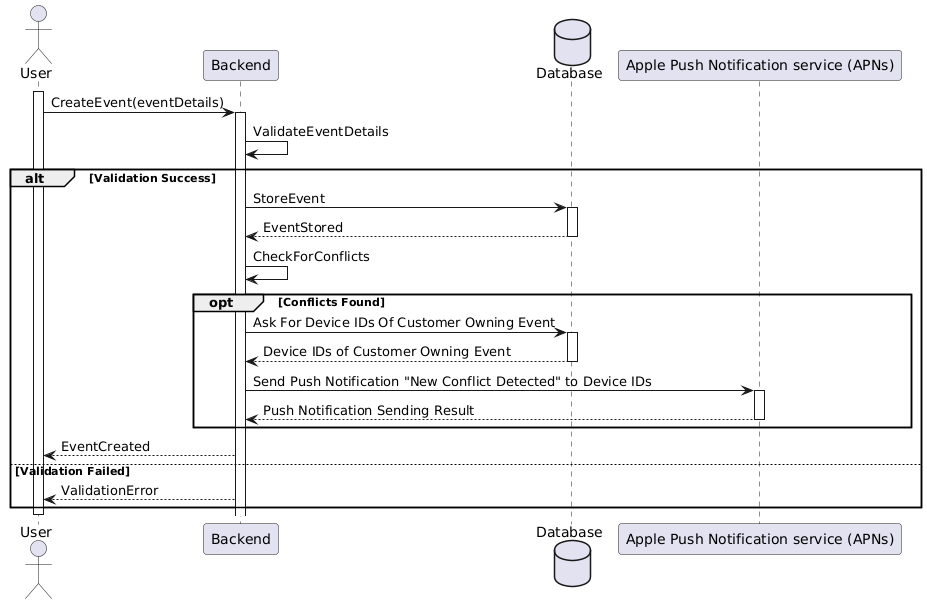
\includegraphics[width=\textwidth]{images/docs/diagrams/sequence-diagrams/all-sequence-diagrams/Add Event Manually.png}
  \caption{Add Event Manually Sequence Diagram}
  \label{fig:seq/add-event-manually}
\end{figure}

The "Add Event Manually Sequence Diagram", shown in \textbf{Figure~\ref{fig:seq/add-event-manually}}, illustrates the process flow when a user manually creates a new calendar event. The sequence begins when the user submits event details through the CreateEvent endpoint, triggering a series of validation and storage operations.

The Backend first performs comprehensive validation of the event details, checking for:
\begin{itemize}
  \item Mandatory fields completion (event name, date, time)
  \item Temporal logic (end time after start time)
  \item Format validity of all provided fields
\end{itemize}

Upon successful validation, the system executes the following steps:
\begin{enumerate}
  \item Stores the validated event in the Database
  \item Performs an automatic conflict check with existing events
  \item If conflicts are detected:
        \begin{itemize}
          \item Retrieves the device IDs associated with the event owner
          \item Dispatches a "New Conflict Detected" notification via Apple Push Notification service (APNs)
        \end{itemize}
  \item Returns an EventCreated response to the user
\end{enumerate}

If validation fails, the system immediately returns a ValidationError to the user, preventing invalid data from entering the system. This workflow ensures data integrity while providing immediate feedback about potential scheduling conflicts, maintaining calendar consistency and user awareness of overlapping appointments.